%%%%%%%%%%%%%%%%%%%%%%%%%%%%%%%%%%%%%%%%%%%%%%%%%%%%%%%%%%%%%%%%%%
%%%%%%%% ICML 2013 EXAMPLE LATEX SUBMISSION FILE %%%%%%%%%%%%%%%%%
%%%%%%%%%%%%%%%%%%%%%%%%%%%%%%%%%%%%%%%%%%%%%%%%%%%%%%%%%%%%%%%%%%

% Use the following line _only_ if you're still using LaTeX 2.09.
%\documentstyle[icml2013,epsf,natbib]{article}
% If you rely on Latex2e packages, like most moden people use this:
\documentclass{article}

% For figures
\usepackage{graphicx} % more modern
%\usepackage{epsfig} % less modern
\usepackage{subfigure} 

% For citations
%\usepackage{natbib}
%\usepackage{gensymb}

%\usepackage{biblatex}
%\addbibresource{sample.bib}

% For algorithms
\usepackage{algorithm}
\usepackage{algorithmic}
\usepackage{amsmath}

% As of 2011, we use the hyperref package to produce hyperlinks in the
% resulting PDF.  If this breaks your system, please commend out the
% following usepackage line and replace \usepackage{icml2013} with
% \usepackage[nohyperref]{icml2013} above.
\usepackage{hyperref}

% Packages hyperref and algorithmic misbehave sometimes.  We can fix
% this with the following command.
\newcommand{\theHalgorithm}{\arabic{algorithm}}

% Employ the following version of the ``usepackage'' statement for
% submitting the draft version of the paper for review.  This will set
% the note in the first column to ``Under review.  Do not distribute.''
%\usepackage{icml2013} 
% Employ this version of the ``usepackage'' statement after the paper has
% been accepted, when creating the final version.  This will set the
% note in the first column to ``Proceedings of the...''
\usepackage[accepted]{icml2013}

\linespread{1}


% The \icmltitle you define below is probably too long as a header.
% Therefore, a short form for the running title is supplied here:
\icmltitlerunning{Predicting Forest Fires Using Multivariate Regression}

\begin{document} 

\twocolumn[
\icmltitle{Predicting Forest Fires Using Multivariate Regression}

% It is OKAY to include author information, even for blind
% submissions: the style file will automatically remove it for you
% unless you've provided the [accepted] option to the icml2013
% package.
\icmlauthor{Alexander Powell, Nathaniel Chien, David McPherson}{ajpowell@email.wm.edu, npchien@email.wm.edu, dfmcpherson@email.wm.edu}

% You may provide any keywords that you 
% find helpful for describing your paper; these are used to populate 
% the "keywords" metadata in the PDF but will not be shown in the document
\icmlkeywords{boring formatting information, machine learning, ICML}

\vskip 0.3in
]

\begin{abstract} 
A growing concern across much of the western United States is the risk of forest fires due to both human negligence and an increasingly dry climate. Detection of regions at high risk of burning and of the potential extent of damages goes a long way in future prevention and control of these “wildfires”. Metrics such as weather, time of day, and population density can be utilized to predict where and how extreme a forest fire will be. Our project aims to apply machine learning techniques, primarily multivariate regression, to predict the burned area of known fires using weather conditions as features. Multiple different regression analyses (e.g. OLS, Lasso, Ridge, Elastic.Net, etc.) will be run and compared for their predictive success. This approach will provide a recommendation for future methodology to predict at-risk-areas based on current meteorological conditions.
\end{abstract} 

\section{Motivation}

Forest fires, commonly referred to as wildfires, are a natural part of many ecosystem cycles. They are an important control on vegetative growth in forests around the globe (Cochrane, 2009). However, the risk of property damage from uncontrolled fires and the threat they can pose to human safety has made their suppression an important part of human ecosystem maintenance. The threat of wildfire damage has become an even more pertinent issue in recent years due to human expansion into areas at high wildfire risk (Lee, 2015). That, combined with recent evidence linking increased wildfire potential with man-made climate change has increased the demand for predictive models of fire extent and damage. The scientific community has thrown itself behind understanding the changes in forest fire intensity and frequency within the coming decades [Fig. 1].

\begin{figure}[!ht]
\centering 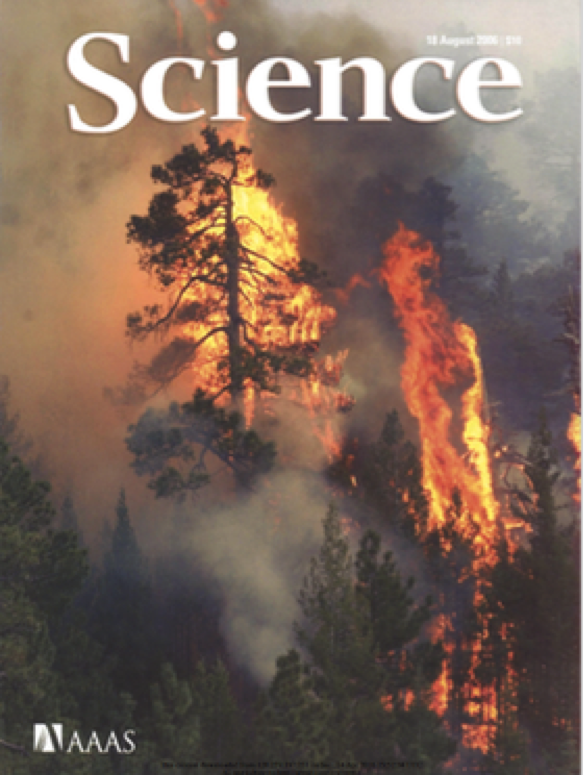
\includegraphics[width=0.3\textwidth]{images/aaas_cover.png}
\caption{The 2006 Cover of Science, a prominent American research journal.}
\end{figure}

Global climate change is expected to stress ecosystems around the world due to changes in temperature, precipitation and other climate attributes such as intensity and frequency of atypical climate events (Cochrane, 2009). A 2007 IPCC report predicts temperatures to rise by 1.8-4.0$^{\circ}$ C by 2100. These changes along with predicted fluctuations in regional precipitation will result in many wildlife habitats, even those historically resistant to fire spread, seeing an increase in wildfire intensity and damage (Uhl \& Kauffman, 1990). Some of these ecosystems include the dense canopied jungles of the Amazon, the Alaskan boreal forest and even Yellowstone National Park within the United States, to name a few (Cochrane, 2009; Johnstone, 2010; Westerling, 2011). 

Protected parks, often the most heavily monitored regions for wildfire potential, are at the forefront of fire prediction modeling (Jahdi, 2015). One such model focused on Golestan National Park in Iran used weather, land cover, and topographic features to predict percentage of burned areas from historical fires in the park and then compared their results to the known fire extent with high predictive success (Jahdi, 2015). As accurate as these models can be, oftentimes they suffer simply from a lack of pre-fire data. A similar study linking climate change models with fire damage prediction models was performed in Yellowstone (Westerling, 2011). Their findings predict a dramatic change in ecosystem processes, flaura and fauna by the middle of this century. Fires in this region of the United States are expected to require less time to burn more area (Westerling, 2011). Following the consensus that forest fires will have an increasing threat on the remaining global biodiversity, this project aims to apply machine-learning techniques to predict the extent of burned area caused by wildfires. 

\begin{figure}[!ht]
\centering 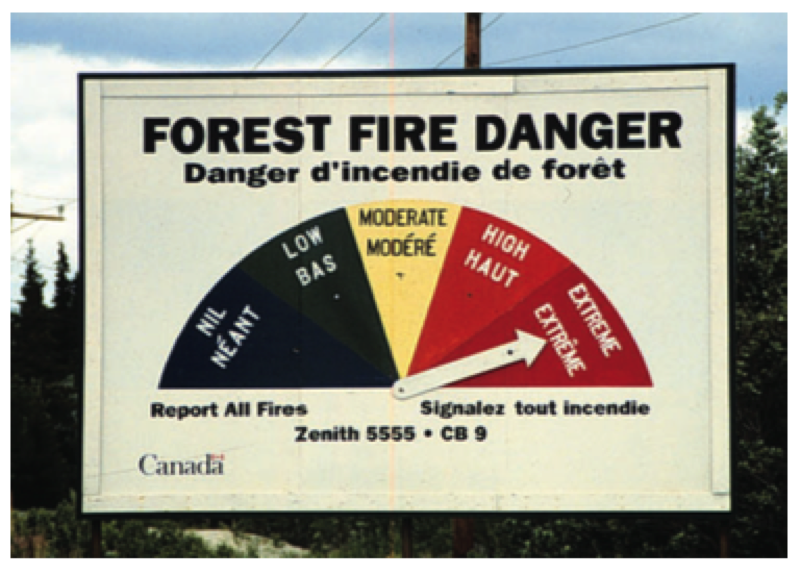
\includegraphics[width=0.45\textwidth]{images/fire_poster.png}
\caption{A fire danger indicator from the Yukon Territory, Canada. Photography by AK Beaver, Yukon Wildland Management.}
\end{figure}

Rating systems [Fig. 2] are one of the most common ways to evaluate forest fire potential on any given day. Common systems include the US National Fire Danger Rating System, the McArthur fire danger meters used in Australia, and the Canadian Forest Fire Danger Rating System (Taylor, 2006). All rating systems try to synthesize the scientific communities understanding of fire risk into a prediction of fire danger. While these systems rely on a number of different metrics to create a succinct judgment on fire risk, the main constituents of a fire rating system are the weather conditions preceding the fire. These include air moisture, wind, humidity, etc. The Canadian Forest Fire Weather Index (FWI) is one way to aggregate these variables and link them to a numerical value that can be used in quantitative fire prediction models [Fig. 3]. 

\section{Data \& Features}

The data set we are using for our regression task comes from the Tras-os-Montes northeast region of Portugal, in the Montesinho natural park.  In total, it contains 517 observations and 13 features.  The data from this set was collected from January 2000 to December 2003.  The 12 input features and 1 output features are described below:
\begin{enumerate}
\item x-axis spatial coordinate within the Montesinho park map: 1 to 9
\item y-axis spatial coordinate within the Montesinho park map: 2 to 9
\item Month of the year: ``jan" to ``dec" 
\item Day of the week: ``mon" to ``sun"
\item FFMC index from the FWI system: 18.7 to 96.20
\item DMC index from the FWI system: 1.1 to 291.3 
\item DC index from the FWI system: 7.9 to 860.6 
\item ISI index from the FWI system: 0.0 to 56.10
\item Temperature in Celsius degrees: 2.2 to 33.30
\item Relative humidity in \%: 15.0 to 100
\item Wind speed in km/h: 0.40 to 9.40 
\item Outside rain in mm/m2 : 0.0 to 6.4 
\item The burned area of the forest (in ha): 0.00 to 1090.84 
\end{enumerate}

It makes sense that many of these features may be correlated, so we knew we would be performing some type of multivariate regression on the dataset.  The four fire danger indices in the features come from the forest Fire Weather Index (FWI) which is the Canadian system for rating fire danger.  Fine Fuel Moisture Code (FFMC), Duff Moisture Code (DMC), and Drought Code (DC) are all related to fuel codes.  FFMC is a numerical rating of the moisture content of litter and other cured fine fuels.  This code is an indicator of the relative ease of ignition and flammability of fine fuel.  DMC is a numerical rating of the average moisture content of loosely compacted organic layers of moderate depth.  It gives an indication of fuel consumption in moderate duff layers and medium-size woody material.  DC is another numerical rating of the average moisture content of deep, compact, organic layers.  This code is a useful indicator of seasonal drought effects on forest fuels, and amount of smouldering in deep duff layers and large logs.  Additionally, the Initial Spread Index (ISI) is a numerical rating of the expected rate of fire spread.  It combines the effects of wind and FFMC on rate of spread without the influence of variable quantities of fuel [Fig.].  

\begin{figure}[!ht]
\centering 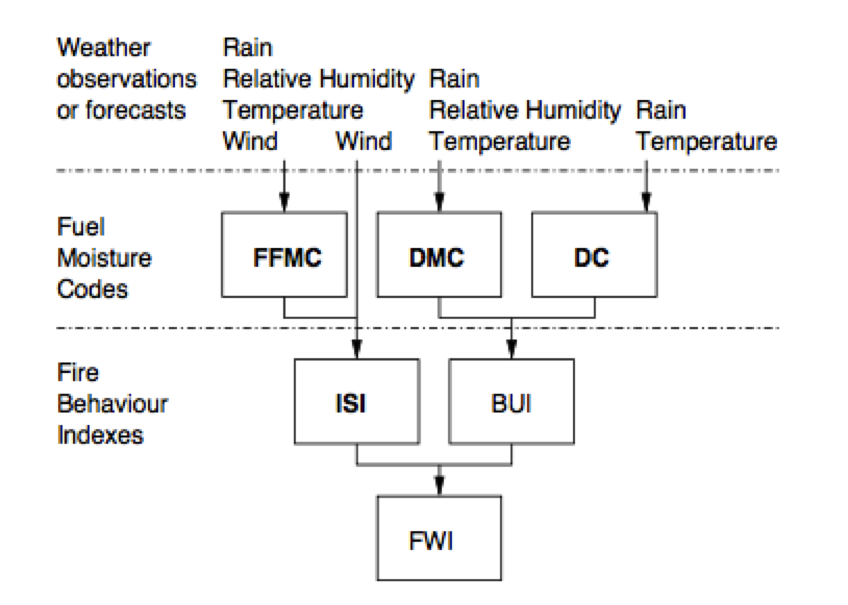
\includegraphics[width=0.5\textwidth]{images/fwi_chart.png}
\caption{A map of the relationships between different forest fire indices. Modified from Taylor, 2006.}
\end{figure}

The data was collected over a span of almost 4 years.  Between January 2000 and December 2003, every time a forest fire occurred, several features were recorded.  The temperature, humidity, and wind speed were all recorded at the time the fire was discovered.  The rain variable denotes the accumulated precipitation within the previous 30 minutes.  The output variable, burned area (in ha), was always measured when a fire had occured.  However, there are a great deal of entries (almost half), with a burned area of 0 ha.  A zero value means that an area lower than 100$m^2$ was burned.  Because so many entries are 0 or a relatively small number, it makes more sense to apply a logarithmic function to the data in order to reduce skewness and improve symmetry.  In the case of this data set, the logarithm function
$$ y = ln(x+1) $$
was used.  

We suspected that a number of these features may be correlated, but it wasn't immediately obvious which features to select.  Python's seaborn library was imported to get some sense of which features were correlated, in an effort to narrow a feature selection a bit.  In the end, features 5 through 12 were selected as they returned the lowest root mean squared error (RMSE).  The $x$ and $y$ axis were not included in the regression as they would limit the potential of the model to the Montesinho park, and the hope for this project is to be able to apply data from any region of somewhat similar climate, to predict and prevent forest fires.  Additionally, the month and day features were excluded from the model.  Initially, it made sense to include them as most forest fires are caused by humans, and humans tend to start fires during the weekend as opposed to the work week.  Additionally, fires are more prevalent during vacation seasons.  However, after some initial regression tests, we found our model did a better job at predicting fires without these features. 

\section{Methodology}

Initially, we ran our data set through an ordinary least squares regression model in an attempt to predict the output variable, burned area.  In the first instance we used only features 5 through 8 (FFMC, DMC, DC, ISI).  Next we used features 9 through 12 (temperature, relative humidity, wind speed, and rain).  Finally, we ran our data set with all 8 features together.  What we found wasn't exactly what we had hoped.  Our initial results did not find much correlation between the any of the input variables and the response variable.  To combat this, we took another look another look at our feature selection.  Initially, the month and day features were left out as they weren't numerical quantities.  However, the vast majority of forest fires are caused by humans, so it made sense that they would be more prevalent during weekends when people were vacationing or enjoying the park.  Also, forest fires are probably more common in the summer than the winter, since more people are on vacation.  Additionally, the hot summer months dry out the dead leaves and other fuel that fires need to grow.  As described above, these were modified to be binary variables so that they could be incorporated into the report.  

Also, the $x$ and $y$ park coordinates were not included in the initial regression model, as they made our findings less practical for other parks around the globe to utilize.  However, they were included due to the low correlation coefficients that were being produced.  

Ultimately, we ended up with 12 features to use to predict the likelihood of a forest fire in the Montesinho national park.  Most of these features were continuous, but several were discrete (Month of the year, day of the week).  Because we had a number of features to predict one response, multivariate regression seemed like a logical choice.  The first method performed on the data set was ordinary least squares regression.  This was done to get a sense of how well the features were correllated more than anything.  Additionally, we performed Ridge and Lasso Regression as well as Elastic.NET regression.  \\ \\ \\ \\ \\

\section{Results}

\subsection{Regression Models}

We performed four regression methods with the data, Ordinary Least Squares (OLS), Ridge, Lasso, and Elastic Net.
Ordinary Least Squares (OLS) is a widely used type of regression. It estimates parameters using least squares, which is done by minimizing the function 
$$ J(\theta) = \dfrac{1}{2m}\sum_{i = 1}^{m} \big( y^{(i)} - \hat y^{(i)}  \big)^2 $$
where m is the number of observations, $y$ is the actual observation, and $y^{\wedge}$ is the predicted value using the current coefficients of the model. By minimizing the squares of differences between $y$ and $y^{\wedge}$ we are finding the best fit given the current data.
A good regression model is one that can make accurate predictions. OLS is known to perform poorly in real-world prediction, and thus improvements have been proposed to its method. If a feature has a small value compared to its coefficient, the coefficient can end up driving estimates. So the improvements involve the use of a penalization piece added to the OLS function, which serves to shrink coefficients.
Ridge regression is one of these methods. Ridge regression adds the square of the L2-norm to OLS as a penalty. By adding it to the function to minimize, the coefficients are then also minimized. A tuning parameter (lambda) is used to give the L2-norm more or less weight when doing Ridge Regression. Since the tuning parameter is the same for each coefficient, the features must be normalized to ensure none of them are being shrunk unfairly. Ridge can also be thought of as minimizing the OLS while keeping the L2-norm below some constant.
Lasso Regression is another method used to shrink coefficients beyond what OLS would give. It is similar to Ridge Regression in this regard, but instead of the L2-norm it includes the addition of the L1-norm. By doing so it enables not only shrinkage of the coefficients, but also variable selection. It will select at most m variables (where m is the number of observations). Like Ridge Regression, Lasso Regression can be thought of as minimizing OLS while keeping the L1-norm below some constant.
Elastic Net Regression is a combination of Ridge Regression and Lasso Regression. It involves both the L2 and L1 norm and has an additional tuning parameter to determine what percentage to use Ridge versus Lasso Regression.

\begin{center}
\begin{table}
\begin{tabular}{| c | c | c | c | c |}
\hline
Method & OLS & Ridge & Lasso & Elastic.Net \\
\hline
%$R^2$ & $0.038$ & N/A & N/A & N/A \\
RMSE & $92.03$ & $90.61$ & $91.04$ & $91.04$ \\
MAE & $22.91$ & $22.35$ & $21.56$ & $21.56$ \\
Lambda & N/A & $10$ & $10$ & $10$ \\
\hline
\end{tabular}
\\
\caption{Results of different regression models on entire data set. Note: RMSE is root mean squared error and MAE is mean absolute error.}
\end{table}
\end{center}

\begin{center}
\begin{table}
\begin{tabular}{| c | c | c | c | c |}
\hline
Method & OLS & Ridge & Lasso & Elastic.Net \\
\hline
%$R^2$ & $0.055$ & N/A & N/A & N/A \\
RMSE & $46.06$ & $39.42$ & $36.64$ & $36.59$ \\
MAE & $30.08$ & $27.39$ & $26.49$ & $26.59$ \\
Lambda & N/A & $10$ & $10$ & $10$ \\
\hline
\end{tabular}
\\
\caption{Results of different regression models on observations from data set with fires over $100m^2$. Note: RMSE is root mean squared error and MAE is mean absolute error.}
\end{table}
\end{center}

\begin{figure}[!ht]
\begin{flushright}
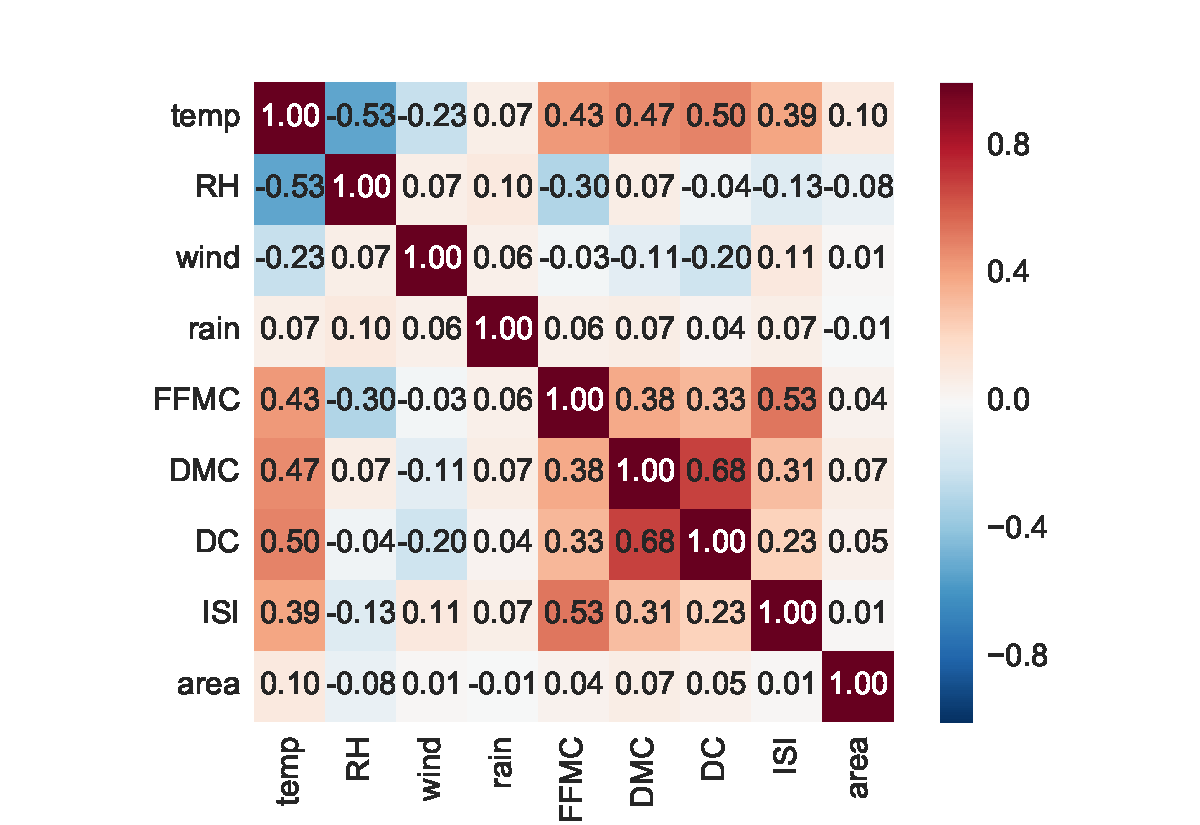
\includegraphics[width=0.5\textwidth]{images/corr_mat.pdf}
\caption{Correlation Matrix of all features.}
\end{flushright}
\end{figure}

\begin{figure}[!ht]
\begin{flushright}
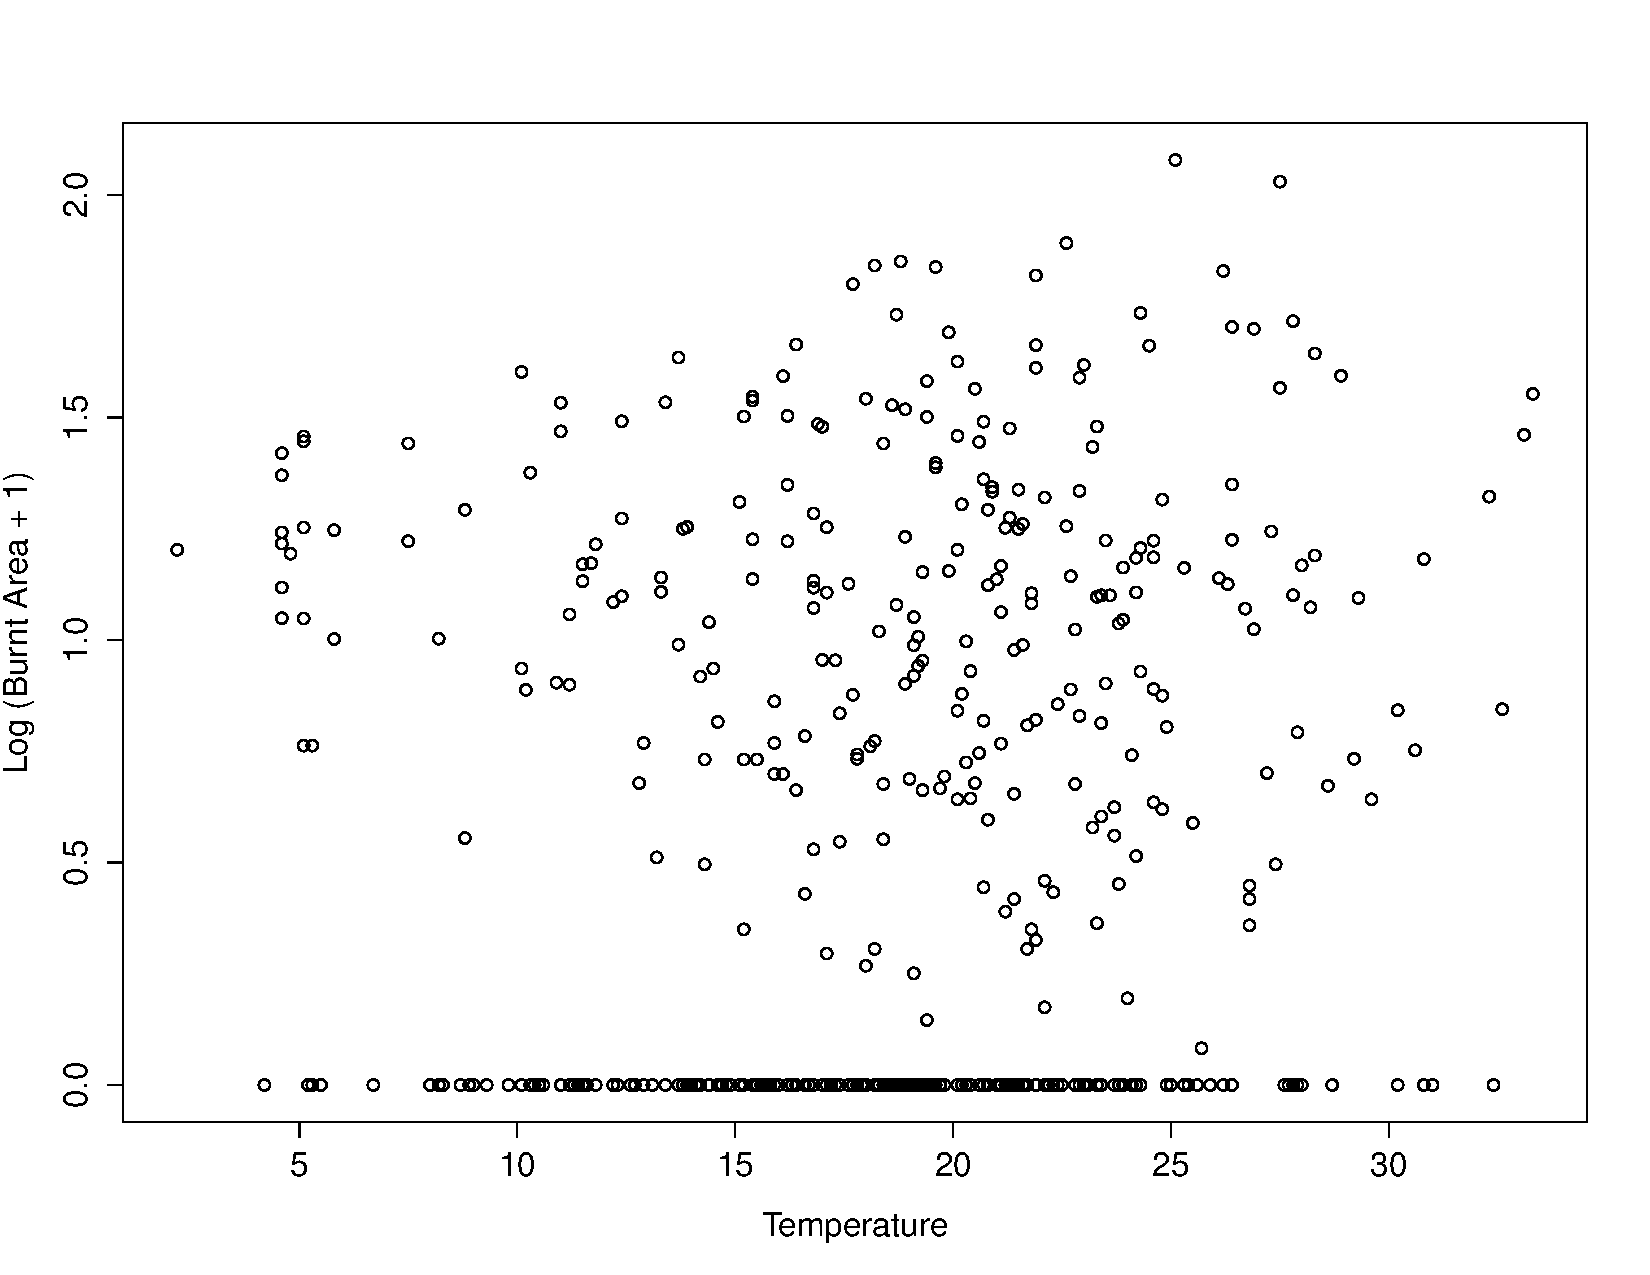
\includegraphics[width=0.5\textwidth]{images/temperature.pdf}
\caption{Scatterplot to show relation between temperature at time of fire and size of area burned.}
\end{flushright}
\end{figure}

\subsection{Analysis}

Table 1 shows the results of our regression algorithms for the four main methods, ordinary least squares, ridge, lasso and elastic net using all of the features provided in the dataset. Table 2 is similar except it uses only the observations that have non-zero burned areas. The OLS $R^2$  for all the data, including data with zero burn area, was 0.038. By eliminating the data with zero burn area (so less than 100 $m^2$) we obtained an $R^2$ of 0.055, indicating that the burn area was more linearly correlated with the features after this elimination.  All four regression techniques had very similar results. Ridge Regression had the lowest root mean squared error while ordinary least squares, the simplest algorithm, had the highest. However, there really wasn’t significant deviation between the errors. Mean Absolute Error shows a similar trend. Table 2 is more clear cut with error decreasing from ridge to lasso to elastic net. Root mean square error decreased significantly going from table 1 to 2. However, Mean absolute error increased in all four cases. This last trend indicates that the forest fire area was not the main reason for the poor performance of these regression techniques.

Comparing our results to that of others who have worked on this project highlights the general poor correlation inherent in the dataset. While Cortez and Morais (2007) did have reduced Mean Absolute Errors (within the 10-20 range) their root mean squared error was still quite high (~65 on average). These results are somewhat meaningless without context however, looking at the correlation between burned area and each feature one begins to get a better picture of the poor relationships inherent in the dataset. The correlation matrix shown earlier highlight this fact. The feature that had the highest correlation with burned area was temperature and it only had 0.10. 

\subsection{Classification Approach}

It is possible that atmospheric conditions do not play a significant role in the extent that a fire reaches. Or that atmospheric conditions only come into play once a fire reaches a certain area that human intervention is unlikely to be a major control on their size. We tested this hypothesis by changing our approach from a regression problem to a classification one. We ran multiple tests converting the burned area to a 0 or a 1 depending on whether the fire area exceeded a certain threshold. Our prediction success, using all of the variables as features, can be seen in Table 3. Classification accuracy increases dramatically the larger the threshold area is. This could be in part due to the smaller number of fires that reach those large areas or it could be related to atmospheric conditions playing a bigger role in creating uncontrollable fires.

\begin{center}
\centering
\begin{table}
\begin{tabular}{| c | c | c |}
\hline
Threshold & Number of & Classification \\
Area($km^2$) & fires above & Accuracy \\
 & threshold area & \\
\hline
$>0$ & $270$ & $51\%$ \\ 
$>1$ & $243$ & $48\%$ \\ 
$>10$ & $95$ & $74\%$ \\ 
$>50$ & $24$ & $94\%$ \\ 
$>100$ & $11$ & $97\%$ \\
\hline
\end{tabular}
\\
\caption{Results from Classification with Logistic Regression}
\end{table}
\end{center}

\section{Conclusion}

Our results indicate that atmospheric conditions alone are not a good predictor of the extent of burned area. One potential reason for the poor correlation between atmospheric conditions and the extent of burned areas is that humans are likely the major control on fire size. After a fire reaches a certain extent, where fire risk to human life and property is likely, local authorities usually step in and take steps to control the fire. If abnormally dry conditions persist for an extended period of time then fire extent could potentially be predicted better. In this scenario, a fire would be more likely to burn large swaths of area. Furthermore humans have less control when fires reach a certain point. This holds true with our classification results.

While it is unlikely that atmospheric conditions play no role whatsoever in controlling a fire’s extent, it is likely that atmospheric conditions are not particularly relevant to this particular study area, Montesinho Natural Park. Fire relies on an external force to start, either natural (e.g. lightning) or man made (e.g. accident). The ratio of these two fire starters is known to vary spatially (as well as temporally). In Canada fires are predominantly due to lightning whereas in the western United States fires are far more likely to be started by humans. The atmosphere likely plays a larger role in creating natural fires and in regions like the boreal forest of the Arctic, this multivariate regression approach may predict fire extent better.

This project was a great example of how machine learning algorithms cannot be used for every data set in existence. The poor correlation found throughout all attempted methodologies is a good indicator. In retrospect, better and earlier use of exploratory data analysis would have helped to evaluate the practicality of this data mining approach. However, the project as a whole was a good lesson in how data analysis cannot be forced onto a dataset. Natural trends do need to exist for meaningful insight to be gained.

\section{References}

\begin{enumerate}

\item
Cochrane, M. A. and Barber, \emph{C. P. Climate change, human land use and future fires in the Amazon. Global Change Biology},
\hskip 1em plus
  0.5em minus 0.4em\relax v. 15 p. 601-612, 2009.\\

\item
P. Cortez and A. Morais. \emph{A Data Mining Approach to Predict Forest Fires using Meterological Data. }
\hskip 1em plus
  0.5em minus 0.4em\relax December, Guimaraes, Portugal, p. 512-523, 2007.\\

\item
Neves, J., Santos, M. F., and Macahdo, J. \emph{New Trends in Artificial Intelligence, Proceedings of the 13th EPIA 2007 – Portuguese Conference on Artificial Intelligence},
\hskip 1em plus
  0.5em minus 0.4em\relax December, Guimaraes, Portugal, p. 512-523, 2007. \\

\item
Solomon S, Qin D, Manning M, Chen Z, Marquis M, Averyt KB, Tignor M, Miller HL \emph{IPCC (2007) Climate change 2007: the physical science basis. In: Contribution of Working Group I to the Fourth Assessment Report of the Intergovernmental Panel on Climate Change},
\hskip 1em plus 
  0.5em minus 0.4em\relax pp. 1–996. IPCC, Cambridge, UK and New York, NY, USA. \\

\item
Jahdi, R., Salis, M., Darvishsefat, A. A., Alcasena, F., Mostafavi, M. A., Etemad, V., Lozano, O. M., and Spano D. \emph{Evaluating fire modeling systems in recent wildfires of the Golestan National Park, Iran.}
\hskip 1em plus
  0.5em minus 0.4em\relax Forestry, v. 0, p. 1-14, 2015. \\

\item
Johnstone, J. F., Hollingsworth, T. N., Chapin, F. S., and Mack, M. C. \emph{Changes in fire regime break the legacy lock on successional trajectories in Alaskan boreal forest.}
\hskip 1em plus
  0.5em minus 0.4em\relax Global Change Biology, v. 16, p. 1281-1295, 2010. \\

\item
Lee, C., Schlemme, C., Murray, J., Unsworth, R. \emph{The cost of climate change: Ecosystem services and wildland fires.}
\hskip 1em plus
  0.5em minus 0.4em\relax Ecological Economics, v. 116, p. 261-269, 2015. \\

\item
Taylor, S. W. and Alexander, M. E.  \emph{Science, technology and human factors in fire danger rating: the Canadian Experience.}
\hskip 1em plus
  0.5em minus 0.4em\relax International Journal of Wildland Fire. v. 15, p. 121-135, 2006. \\

\item
Uhl C., Kauffman J. B. \emph{Deforestation, fire susceptibility, and potential tree responses to fire in the eastern Amazon.}
\hskip 1em plus 
  0.5em minus 0.4em\relax Ecology, v. 71, p. 437–449, 1990. \\

\item
Westerling, A. L., Hidalgo, H. G., Cayan,  D. R., and Swetnam, T. W. \emph{Warming and Earlier Spring Increase Western U.S. Forest Wildfire Activity.}
\hskip 1em plus
  0.5em minus 0.4em\relax Science. v. 313, p. 940–943, 2006. \\

\item
Westerling A. L., Turner M. G., Smithwick, E. A. H., Romme W. H., and Ryan, M. G., \emph{Continued warming could transform Greater Yellowstone fire regimes by mid-21st century.}
\hskip 1em plus
  0.5em minus 0.4em\relax PNAS, v. 108, p. 13165-13170, 2011. \\

\end{enumerate}


%\subsection{Submitting Papers}


% In the unusual situation where you want a paper to appear in the
% references without citing it in the main text, use \nocite
%\nocite{langley00}

%\bibliography{example_paper}
%\bibliographystyle{icml2013}

\end{document} 


% This document was modified from the file originally made available by
% Pat Langley and Andrea Danyluk for ICML-2K. This version was
% created by Lise Getoor and Tobias Scheffer, it was slightly modified  
% from the 2010 version by Thorsten Joachims & Johannes Fuernkranz, 
% slightly modified from the 2009 version by Kiri Wagstaff and 
% Sam Roweis's 2008 version, which is slightly modified from 
% Prasad Tadepalli's 2007 version which is a lightly 
% changed version of the previous year's version by Andrew Moore, 
% which was in turn edited from those of Kristian Kersting and 
% Codrina Lauth. Alex Smola contributed to the algorithmic style files.  
